\subsubsection{Attention-Noise Sweep}
\label{app:exp:section5:attn-noise}
The attention-noise experiment in Figure~\ref{fig:ssfr_main_fig}a uses the \emph{pretrained attention} Transformer training setup (Appendix~\ref{app:exp:transformer-setups}) and isolates the attention module during the attention-only pretraining phase.
At evaluation, for each stored key and junk context sampled, we measure the $\ell_2$ deviation between the attention output at the query position and the corresponding stored key embedding. We then aggregate these deviations to estimate the attention noise floor.

We vary junk length
\(
J\in\{2,4,8,16\}
\)
and couple the junk vocabulary size to the length ($V_J=J$).
We run our sweeps using model sizes
\[
(d_{\mathrm{model}},F)\in\{(64,512),(96,1152),(128,2048)\}.
\]
and average over four seeds.

\subsubsection{Noisy-Margin Diagnostic}
\label{app:exp:section5:noisy-margin}
The noisy-margin curve in Figure~\ref{fig:ssfr_main_fig}b
measures how the minimum margin of our bilinear construction changes under perturbed key queries.
We use isotropic keys and values with $d=64$, $F=256$, and hidden width $m=512$.
For each stored key, we perturb it via
\[
\widetilde{\mathbf{k}}_i=\mathbf{k}_i+\epsilon \mathbf{u}_i,
\qquad
\mathbf{u}_i\sim\mathrm{Unif}(S^{d-1}),
\]
and sweep $\epsilon$ logarithmically from $0.01$ to $2.0$ over $15$ values.
For each sweep point, we report the empirical noisy minimum margin and the predicted linear degradation term, averaged over three seeds.

\begin{figure}[h]
\centering
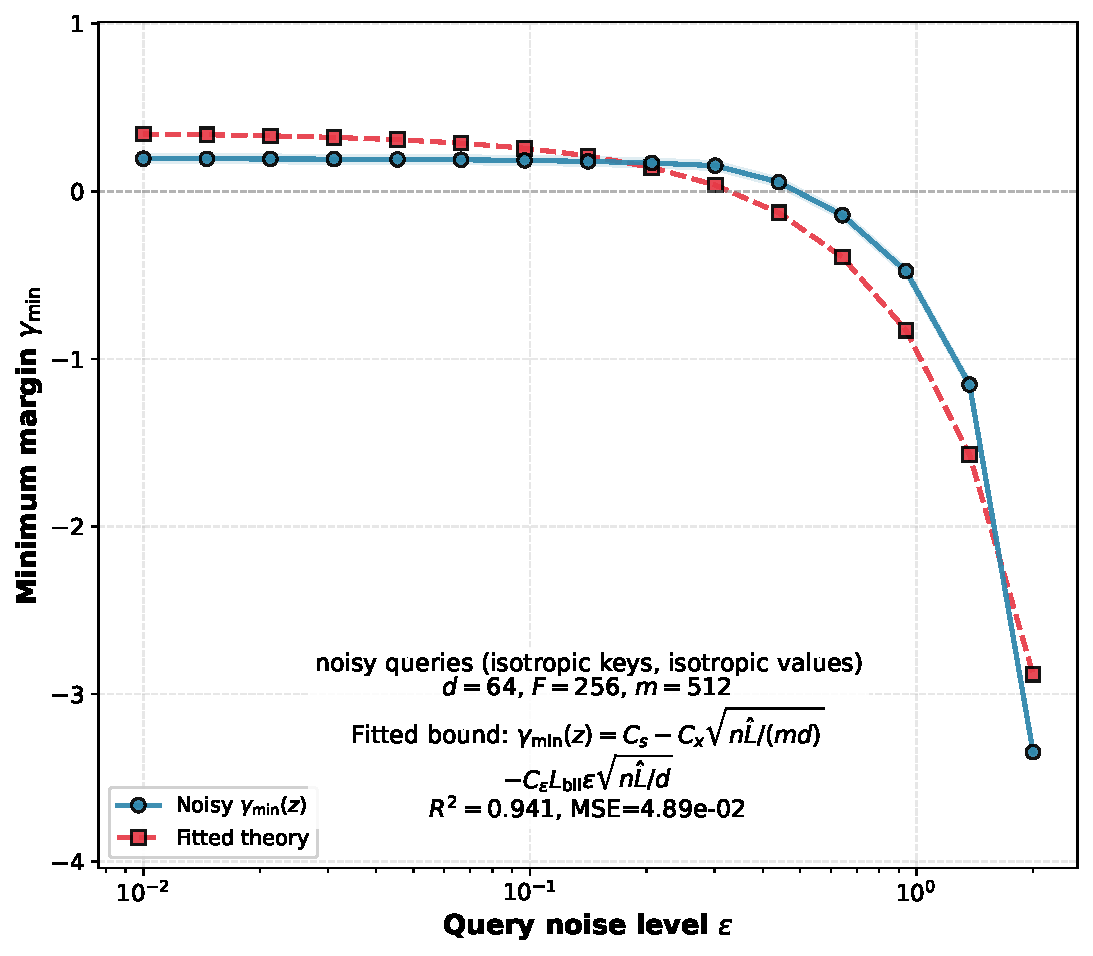
\includegraphics[width=0.60\linewidth]{appendix/theory/margin_sweep_results_aux_epsilon_fit_only.pdf}
\caption{\textbf{Margin degradation under noisy queries.}
Bilinear MLP minimum margin decreases linearly with the magnitude of key perturbations $\epsilon$, validating the noisy-margin degradation bound. The empirical margin (solid line) closely follows the predicted linear degradation term (dashed line) with $d=64$, $F=256$, $m=512$.}
\label{fig:app:noisy-margin-sweep}
\end{figure}

\subsubsection{Transformer Capacity Sweep}
\label{appendix:lm-scaling}

Our Transformer capacity plots use the SSFR task from Appendix~\ref{appendix:ssfr-task} and the \emph{inserted MLP} training setup from Appendix~\ref{app:exp:transformer-setups}. In our experiments, we compare GD, our unwhitened construction, our whitened construction, our data-dependent construction, and the NTK baseline. Unless otherwise stated, we use embedding dimension \(d=128\), junk length \(J=9\), junk vocabulary size \(V_J=9\), \(4{,}000\) training epochs, and one seed.

We evaluate Transformer capacity using two complementary success criteria:
\begin{itemize}
    \item \textbf{Training accuracy.} In this variant, we evaluate a Transformer's accuracy on SSFR using the MLP and the fact set it is trained with. This criterion assesses whether the inserted MLP is well-behaved enough that it can be used inside a Transformer at all. Crucially, this criterion is unable to distinguish between when a Transformer is learning to query its fact-storing MLP to perform factual recall and when it is simply using its attention parameters to memorize the fact set.
    
    \item \textbf{Evaluation (fact-adaptive) accuracy.} In this variant, we train a Transformer using an MLP $MLP_A$ storing a given fact set $A$, but during evaluation, we generate a new fact set $B$ and fact-storing MLP, $MLP_B$, that stores it. We then insert $MLP_B$ into the pretrained Transformer, with no additional training, and evaluate the Transformer's end-to-end accuracy on SSFR \emph {using fact set $B$}.
    This criterion assesses whether the Transformer is performing factual recall by learning to query its fact-storing MLP, while being prevented from introducing additional fact-set-dependent computation.
\end{itemize}

In practice, we find that we need to make two changes to the standard GPT-style architecture to ensure that Transformers trained on a given fact set will learn a fact-adaptive solution: (i) we disable the residual connection after the attention layer to prevent extra signal propagation, and (ii) we freeze the value and output projections to identity matrices to hinder memorization.

For the main-text Transformer-capacity plot in Figure~\ref{fig:main-figure}c, we define Transformer capacity as the smallest model that achieves 100\% fact-adaptive accuracy.
We sweep
\[
F\in\{2^6,2^7,\dots,2^{13}\}=\{64,128,256,512,1024,2048,4096,8192\}
\]
and binary-search over hidden width \(m\in[1,65536]\) with precision \(16\) for each method.

\subsubsection{Per-Key Margin Diagnostic}
\label{app:exp:section5:margin-violin}
The violin plot in \Cref{fig:margin-violin} visualizes the full distribution of per-key margins rather than only the minimum margin, as in the other margin sweeps.
For this experiment, we use the \emph{pretrained attention} setting from Appendix~\ref{app:exp:transformer-setups}.
We use $d=128$, $F=2048$, $J=V_J=9$, $16$ logarithmically spaced hidden widths in $[16,256]$, and four seeds.
For each width, we pool the per-key margins across seeds and compare their distribution against the corresponding combined Transformer accuracy and standalone MLP accuracy.

\begin{figure}[h]
\centering
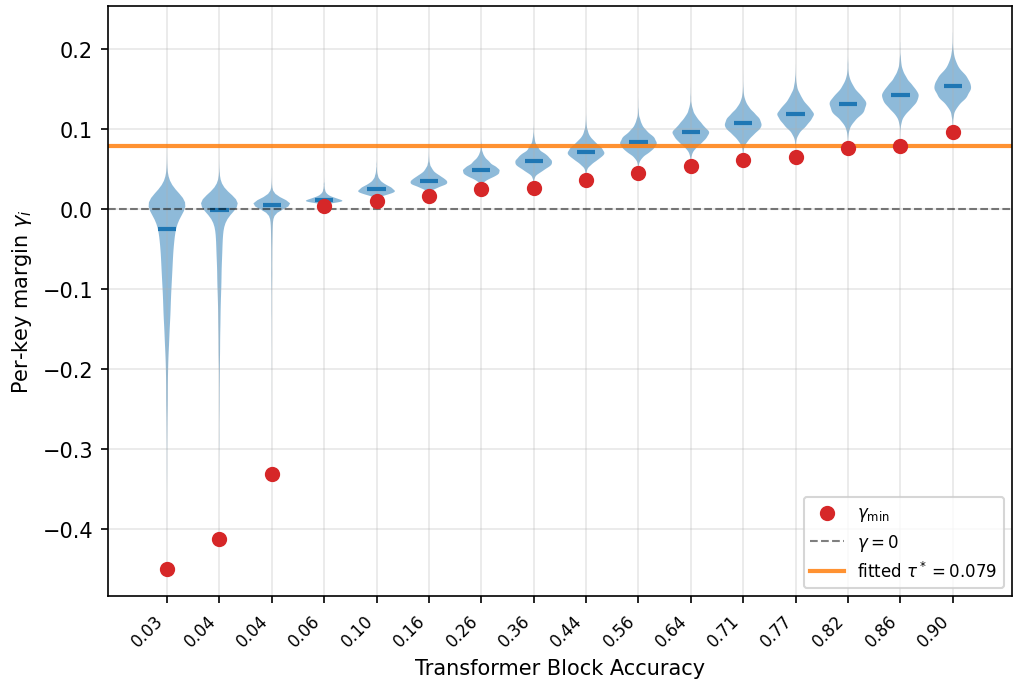
\includegraphics[width=0.62\linewidth]{sections/section_5_transformer_integration/figs/margin_violin.png}
\caption{\textbf{Per-key margin distributions is predictable of end-to-end Transformer accuracy.}
The usable-key fraction inferred from per-key margins is predictable of the combined
attention+MLP Transformer accuracy across the tested models.}
\label{fig:margin-violin}
\end{figure}


\subsubsection{Fact Editing}
\label{appendix:lm-task}
\label{appendix:fact-editing}

\paragraph{Language Modeling Task.}
We introduce a simple language modeling (LM) task to evaluate a Transformer's ability to perform next-token prediction while recalling factual information. In this task, the model is presented with a natural-language sentence expressing a \((\textit{book}, \textit{author})\) relation and is required to predict each subsequent token in the sequence. We curate this dataset using author-book relations from the Goodreads Book Graph Dataset \citep{authors_dataset}.

Formally, let \(f : S_k \to S_v\) be the authors \textit{fact set}, where
\(S_k = \{\text{``It''},\ \text{``1984''},\ \text{``And Then There Were None''},\ \ldots\}\) is the set of book titles (keys) and
\(S_v = \{\text{``Stephen King''},\ \text{``George Orwell''},\ \text{``Agatha Christie''},\ \ldots\}\) is the set of corresponding authors (values).
To simplify analysis, we select exactly one book per author.
Let \(J = \{(\text{``The author of''},\ \text{``is''}),\ (\text{``Who is the author of''},\ \text{``? It is''}),\ \ldots\}\) denote the set of natural-language template prefix--suffix pairs.
The LM task given \(f\) can then be defined as:
\[
    \mathcal{S}_{LM}[f] = \{\text{concat}(t_{\text{prefix}},\ k,\ t_{\text{suffix}}, f(k)) \ |\ (t_{\text{prefix}}, t_{\text{suffix}}) \in J,\ k \in S_k \}.
\]

For example, given the sequence:
\[
\underbrace{\text{The author of}}_{\text{template prefix}}\ 
\underbrace{1984}_{\text{key}}\ 
\underbrace{\text{is}}_{\text{template suffix}}\ 
\underbrace{\text{George Orwell}}_{\text{value}}
\]
from \(\mathcal{S}_{LM}[f]\), the model’s task is to perform next-token prediction \textit{at every position} in the sentence. This LM task allows us to study factual recall in a more natural language modeling setting, complementing the SSFR setup.

\paragraph{Model Parameterization.}
For this experiment, we use a one-layer Transformer architecture with one head and the following non-standard design choices.
We use this parameterization because it was the most
realistic and simplest Transformer variant in our sweep that was able to achieve near-perfect accuracy on the book--author task when trained with an inserted fact-storing MLP.

The model uses frozen tied input/output embeddings, no attention or
MLP residual connection, RoPE positional encoding, freezes the RMSNorm before the MLP, uses an RMSNorm before attention and the language-modeling head, and sets value and output projections of the attention layer frozen to identity matrices. The model hidden dimension is \(d_{\mathrm{model}}=256\).

The attention layer keeps standard causal softmax attention, but uses learned nonlinear query and key projections. If \(z_t\) is the attention-normalized residual stream, then, omitting biases,
\[
  q_t = W_{Q,2}\,\mathrm{GELU}(W_{Q,1}\,\mathrm{LN}(z_t)),
  \qquad
  k_t = W_{K,2}\,\mathrm{GELU}(W_{K,1}\,\mathrm{LN}(z_t)),
  \qquad
  v_t = z_t,
\]
and the attention output is
\[
  a_t=\sum_{s\le t}
  \mathrm{softmax}_{s}\!\left(\frac{q_t^\top k_s}{\sqrt{d_{\mathrm{model}}}}\right)
  v_s,
\]
with the output projection fixed to the identity.

The feedforward layer is a two-expert module. Let \(x_t\) denote the residual stream entering the feedforward block at token position \(t\), and let \(\tilde{x}_t\) be the normalized MLP input after the block's pre-MLP RMSNorm.
The feedforward output is
\[
  \mathrm{FFN}(x_t,\tilde{x}_t)
  =
  \alpha_t f_{\mathrm{fact}}(\tilde{x}_t)
  +
  (1-\alpha_t) f_{\mathrm{aux}}(x_t),
  \qquad
  \alpha_t=\sigma(g_2(\mathrm{GELU}(g_1(x_t)))).
\]
Here \(f_{\mathrm{fact}}\) is the inserted fact-storing MLP, held fixed during Transformer training, and \(f_{\mathrm{aux}}(x)=xUV\) is a trainable rank-\(8\) low-rank linear expert. The router is a two-layer scalar sigmoid MLP that forms a linear combination of the fact expert and auxiliary expert outputs. Intuitively, our goal is for the model to learn to use the fact-storing MLP to store the book--author relations and the auxiliary expert to learn the natural-language sentence formats.

Book titles and author names are added to the model tokenizer as atomic tokens before training. For the fact MLP, the key embedding representing each book is the normalized version of the corresponding atomic book token.

\paragraph{GD MLP Setup.}
In our fact-editing experiment, we use GD-trained fact-storing MLPs (see Appendix~\ref{app:exp:mlp-variant-definitions} for the bilinear gated architecture and optimizer settings), but we train the MLP with a MSE objective under arg-max decoding:
\[
L_{MLP}(\mathbf{K}, \mathbf{V}, f)
\propto
\sum_{i=1}^{|\mathbf{K}|}
\left\lVert
MLP(\mathbf{k}_i) - \mathbf{v}_{f(i)}
\right\rVert_2^2.
\]
The inserted fact expert is a gated MLP with hidden width \(h=512\),
trained by GD for up to \(10{,}000\) epochs with learning rate \(10^{-3}\),
minimum learning rate \(10^{-6}\), and early stopping once the objective falls
below \(10^{-7}\).
Crucially, we train this MLP with MSE rather than cross entropy because MSE
matches the full author-value embedding vectors, not only the nearest-token
classifier. We find that a parameter-matched cross-entropy GD MLP reaches \(100\%\) fact
classification accuracy when evaluated standalone, but when inserted into the Transformer the model reaches only about \(90\%\) accuracy.

\paragraph{Training Setup.}
We train on \(16{,}384\) book-author facts with \(16\) rephrases per fact. We
initialize embeddings with Kaiming-uniform initialization and train the
Transformer with AdamW using learning rate \(2\times10^{-4}\), weight decay
\(0.1\), batch size \(32\), \(18\) epochs, and \(8192\) optimizer steps per epoch.
The trained base reaches near-perfect standalone MLP accuracy \(0.9998\) and Transformer value-token accuracy \(0.9984\).


\paragraph{Evaluation.}
We divide the \(16{,}384\) stored facts into a \emph{preserved} set whose answers should remain unchanged and an \emph{altered} set whose answers are replaced by a fresh permutation of author values.
We edit \(328\), \(819\), or \(1638\) facts, corresponding to \(2\%\),
\(5\%\), and \(10\%\) of the fact set. For altered facts, we evaluate the
new answer on both the edited training template and held-out rephrases; for
preserved facts, we evaluate the original answer.

We report four fact-editing quantities.
\emph{Efficacy} is author-token accuracy on altered facts under the edited labels.
\emph{Paraphrase} is accuracy on held-out rephrasings of the altered facts under the edited labels.
\emph{Specificity} is accuracy on preserved facts under the original labels.
\emph{Score} is the harmonic mean of efficacy, paraphrase, and specificity.
We additionally report the \emph{non-fact PPL ratio}:
\[
  r_{\mathrm{NF}}
  =
  \frac{\mathrm{PPL}_{\mathrm{post,NF}}}{\mathrm{PPL}_{\mathrm{pre,NF}}}
  =
  \exp\!\left(
    \mathrm{CE}_{\mathrm{post,NF}}-\mathrm{CE}_{\mathrm{pre,NF}}
  \right),
\]
where the CE is averaged over all next-token positions except the author-value tokens, across preserved and altered prompts before and after editing.
For example, \(r_{\mathrm{NF}}=1\) means the edit leaves non-fact-token
language-modeling loss unchanged.

\paragraph{Baselines.}
We compare four editing methods:
\begin{itemize}
    \item Our method, \textsc{MLP Swapping}, constructs a replacement GD fact expert for the complete post-edit fact set and swaps that expert into the frozen Transformer, with no update to the surrounding Transformer.
    \item MEMIT~\citep{memit} applies a multi-edit linear residual update to the fact expert's output projection, using altered-fact keys and a regularized solve.
    \item ROME~\citep{rome} applies a rank-one residual update for each edit, adapted to our one-layer setting and applied at the final prompt token.
    \item AlphaEdit~\citep{fang2025alphaeditnullspaceconstrainedknowledge} first estimates a preserve-key subspace and then projects the residual edit into the approximate nullspace of that preserve subspace before updating the fact expert.
\end{itemize}
For the weight-update editors, residuals are computed from a single templated prompt per fact and applied to the inserted MLP output immediately upstream of the logits. We omit random prefix contexts and the ROME KL term because this synthetic dataset has a single relation and a unique author per book.

For each weight-update baseline and edit fraction, we sweep method-specific
hyperparameters and report the score-best configuration. AlphaEdit uses the best targeted grid setting \(\texttt{train\_steps}=100\), \(\texttt{lr}=0.05\), \(\texttt{clip\_norm}=\text{None}\), and \(\texttt{singular\_value\_tolerance}=10\) at all three edit fractions.
MEMIT uses \(\texttt{lr}=0.05\), \(\lambda=150\), and \(\texttt{clip\_norm}=0.75\), with \(100\) steps at \(2\%\) and \(5\%\) edits and \(25\) steps at \(10\%\) edits.
ROME uses \(\texttt{lr}=0.05\), \(\texttt{wd}=1.5\times10^{-3}\), and \(\texttt{early\_stopping\_loss}=5\times10^{-2}\), with \(10\) steps at \(2\%\) edits and \(100\) steps at \(5\%\) and \(10\%\) edits.

\begin{table}[h]
\centering
\scriptsize
\setlength{\tabcolsep}{5pt}
\begin{tabular}{lccccc}
\toprule
Method & Efficacy & Paraphrase & Specificity & Score & \(r_{\mathrm{NF}}\) \\
\midrule
\multicolumn{6}{l}{\(2.00\%\) edited facts} \\
\quad \textsc{MLP Swapping} & \textbf{1.000} & \textbf{1.000} & \textbf{0.999} & \textbf{1.000} & \emph{1.016} \\
\quad AlphaEdit & \emph{0.896} & \emph{0.899} & 0.981 & \emph{0.924} & \textbf{1.000} \\
\quad MEMIT & 0.643 & 0.645 & \emph{0.990} & 0.729 & \textbf{1.000} \\
\quad ROME & \textbf{1.000} & \textbf{1.000} & 0.009 & 0.026 & 1.238 \\
\addlinespace
\multicolumn{6}{l}{\(5.00\%\) edited facts} \\
\quad \textsc{MLP Swapping} & \textbf{0.998} & \textbf{0.998} & \textbf{0.998} & \textbf{0.998} & \emph{1.057} \\
\quad AlphaEdit & 0.747 & 0.745 & 0.909 & \emph{0.794} & \textbf{1.001} \\
\quad MEMIT & 0.128 & 0.126 & \emph{0.986} & 0.179 & \textbf{1.001} \\
\quad ROME & \emph{0.991} & \emph{0.991} & 0.002 & 0.006 & 1.642 \\
\addlinespace
\multicolumn{6}{l}{\(10.00\%\) edited facts} \\
\quad \textsc{MLP Swapping} & \textbf{0.998} & \textbf{0.999} & \textbf{0.999} & \textbf{0.999} & 1.021 \\
\quad AlphaEdit & 0.482 & 0.482 & 0.766 & \emph{0.550} & \emph{1.010} \\
\quad MEMIT & 0.004 & 0.003 & \emph{0.995} & 0.005 & \textbf{1.002} \\
\quad ROME & \emph{0.834} & \emph{0.832} & 0.001 & 0.003 & 2.405 \\
\bottomrule
\end{tabular}
\caption{Fact-editing metrics for baselines and \textsc{MLP Swapping} on the GD MLP base model.
\(r_{\mathrm{NF}}\) is the non-fact-token perplexity ratio.
Bold marks the best value and italics mark the second-best value within each edit fraction and metric; lower is better
for \(r_{\mathrm{NF}}\), and higher is better for all other metrics.
Ties at the displayed precision share the same marking.}
\label{tab:fact-editing-updated-h512}
\end{table}

\begin{figure}[h]
\centering
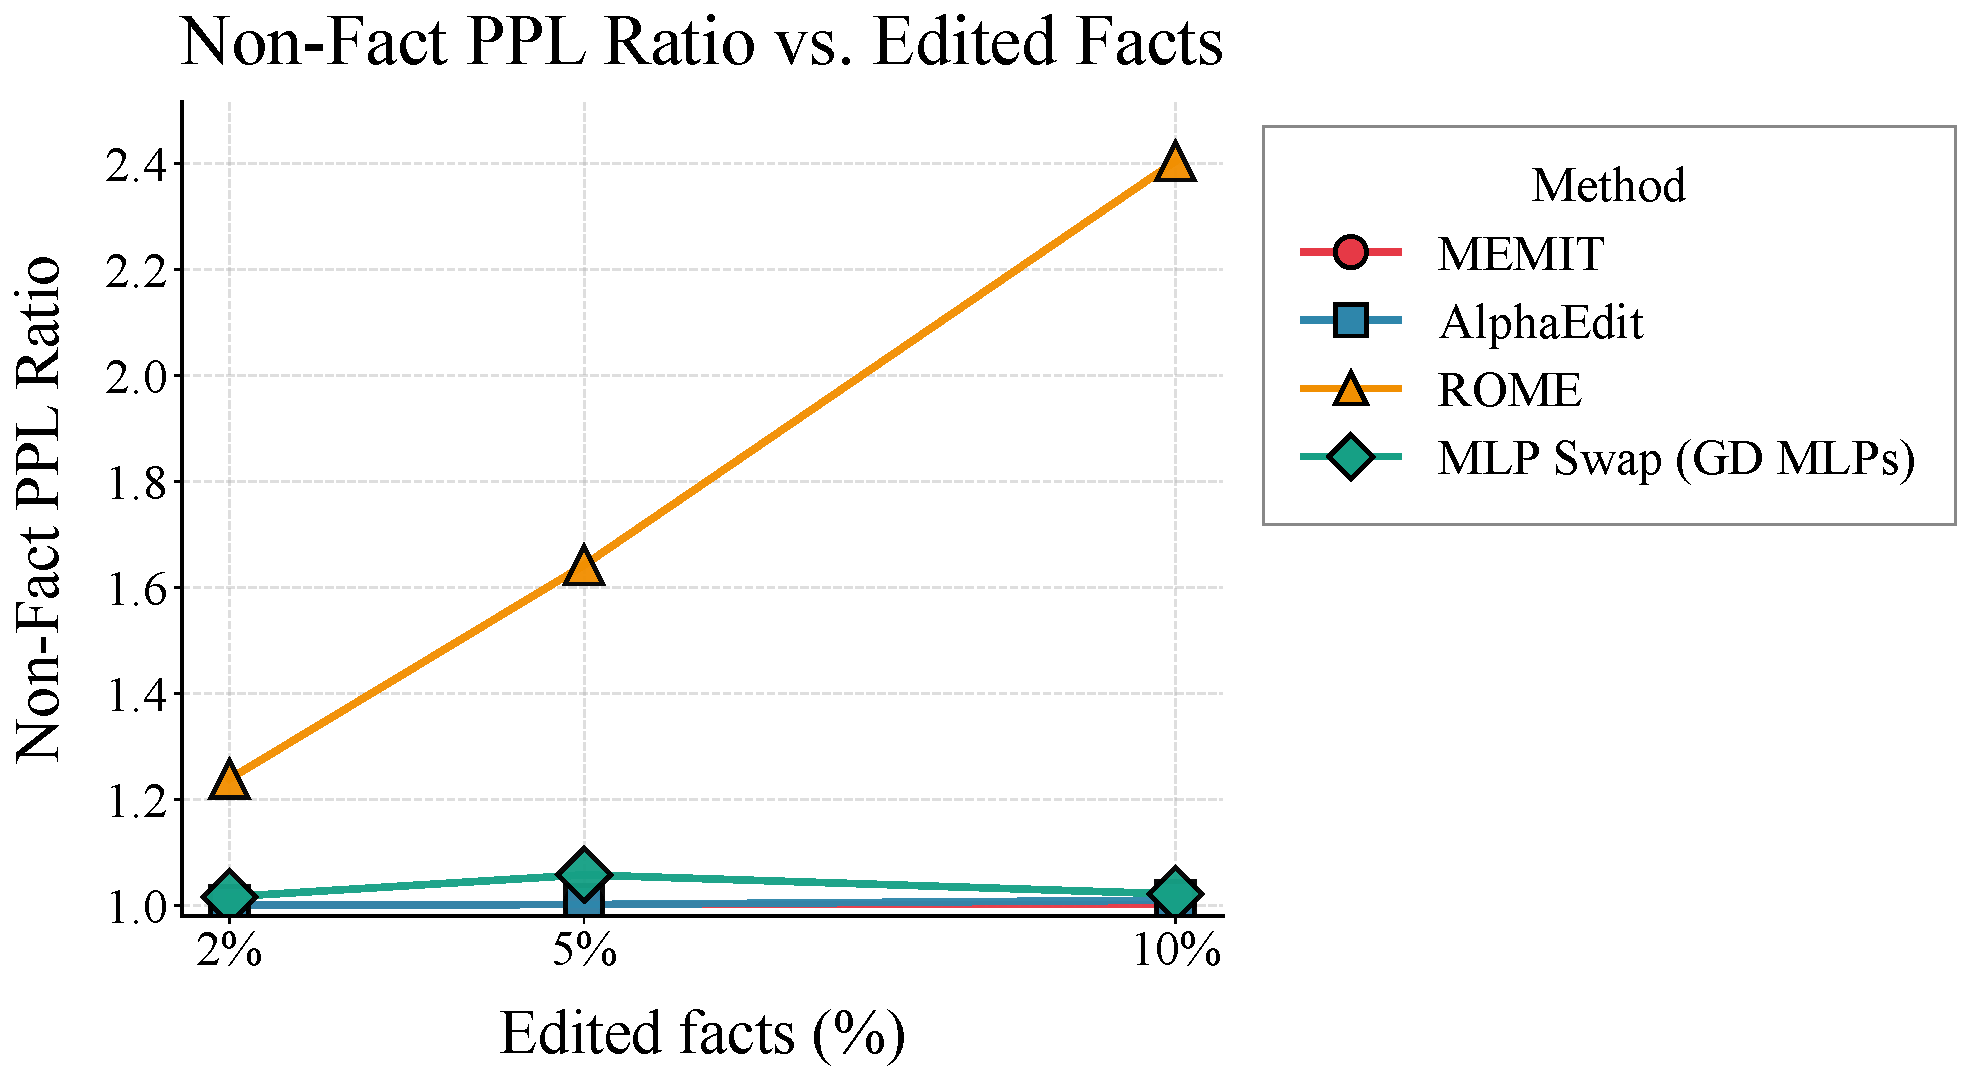
\includegraphics[width=0.68\linewidth]{sections/section_5_transformer_integration/figs/fact_editing_nonfact_ppl_ratio_h512_normtok_mse.pdf}
\caption{Non-fact-token perplexity ratio for the
fact-editing setup of Figure~\ref{fig:ssfr_main_fig}c. AlphaEdit and MEMIT have
nearly unchanged non-fact loss but weaker edit scores at larger edit fractions;
ROME edits target prompts while severely damaging non-fact loss and specificity.
\textsc{MLP Swapping} keeps near-perfect edit scores with a small non-fact PPL
increase, at most \(1.06\times\).}
\label{fig:fact-editing-nonfact-ppl-ratio}
\end{figure}

\paragraph{Fact editing with constructed MLPs.}
We also repeat the fact-editing experiment from Figure~\ref{fig:ssfr_main_fig}c using the \emph{data-dependent Hebbian MLP construction}. Because the data-dependent construction has slightly worse storage capacity scaling than GD MLPs, we find we need to increase the hidden dimension to \(h=1024\) to achieve near-perfect MLP and Transformer accuracy. Other than this change, our experimental setup is the same as described above for GD MLPs.
We retune the method-specific hyperparameters for each of the fact-editing baselines.
We show that \textsc{MLP Swapping} remains effective even with constructed Hebbian MLPs in Figure~\ref{fig:fact-editing-constructed-data-dependent}.
Swapping out a \(h=1024\) data-dependent constructed MLP keeps the edit score above \(0.98\) through up to \(10\%\) edited facts, while the strongest tuned local-editing baseline reaches only \(0.847\) at \(10\%\). The \textsc{MLP Swapping} non-fact PPL ratio remains below \(1.11\times\).

\begin{figure}[h]
\centering
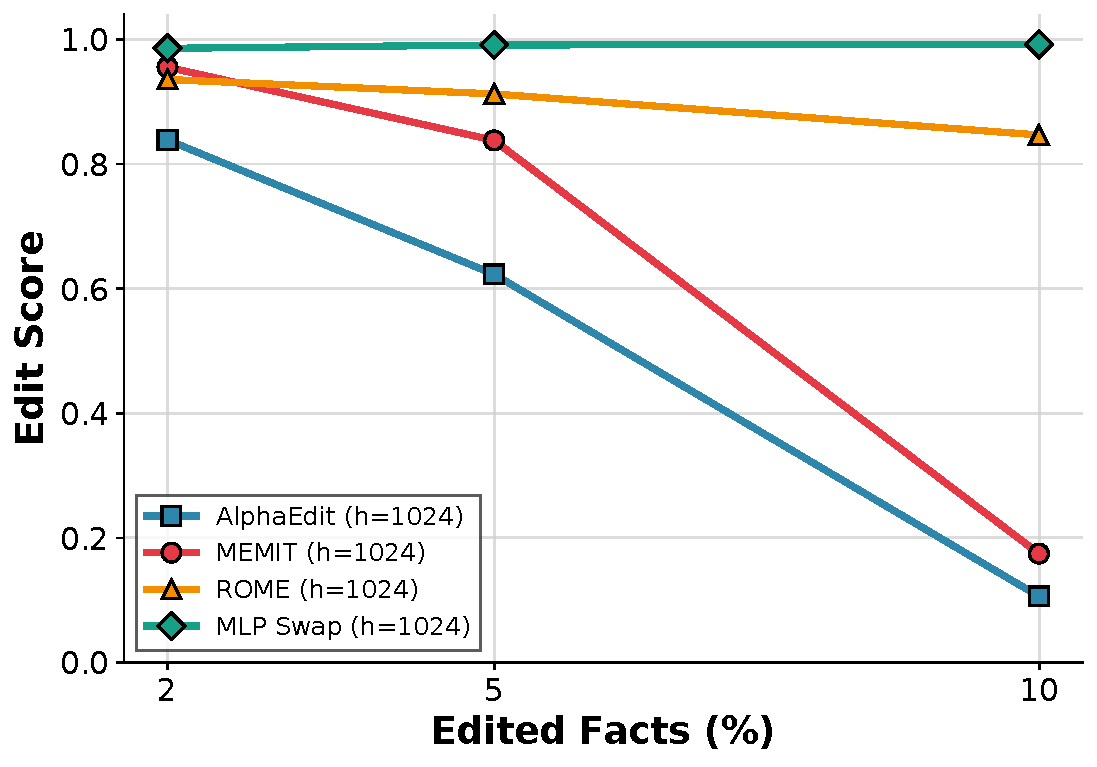
\includegraphics[width=0.68\linewidth]{sections/section_5_transformer_integration/figs/fact_editing_score_constructed_h1024.pdf}\\[0.5em]
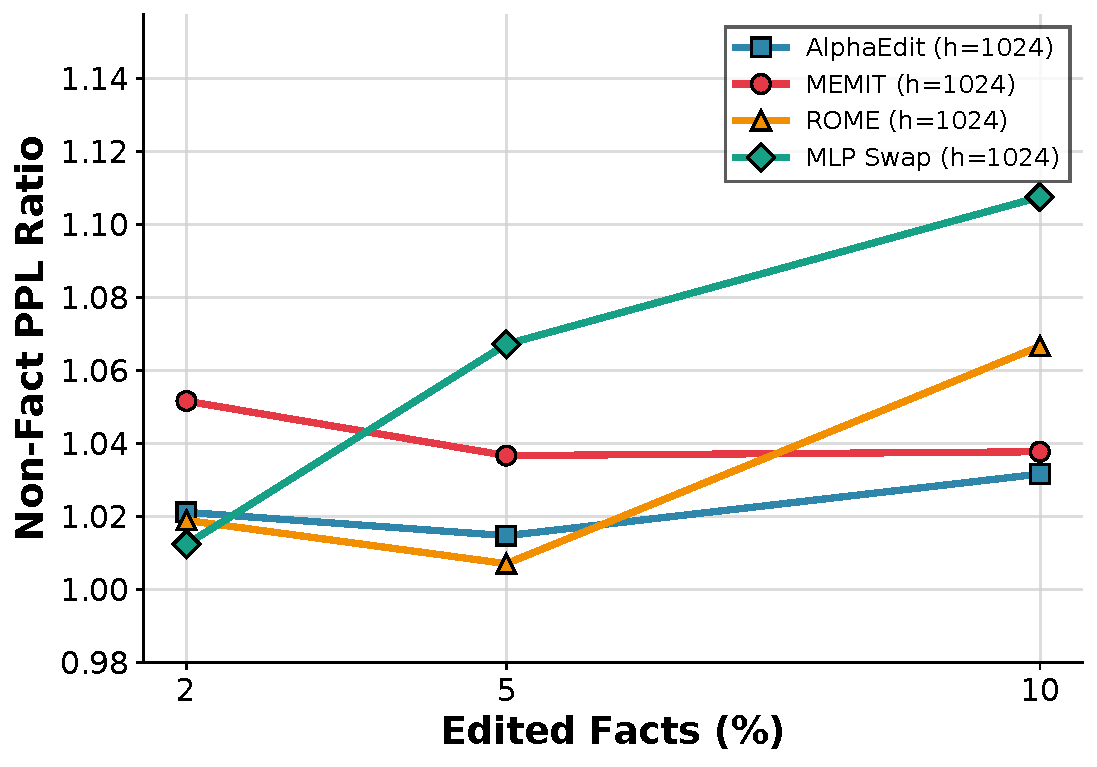
\includegraphics[width=0.68\linewidth]{sections/section_5_transformer_integration/figs/fact_editing_nonfact_ppl_ratio_constructed_h1024.pdf}
\caption{Fact-editing score (top) and non-fact-token perplexity ratio (bottom) for the \(h=1024\) data-dependent constructed-MLP setting. \textsc{MLP Swapping} achieves an edit score above \(0.98\) through up to \(10\%\) edited facts---13 percentage points higher than the next highest baseline---all while non-fact PPL ratio remains below \(1.11\times\).}
\label{fig:fact-editing-constructed-data-dependent}
\end{figure}
